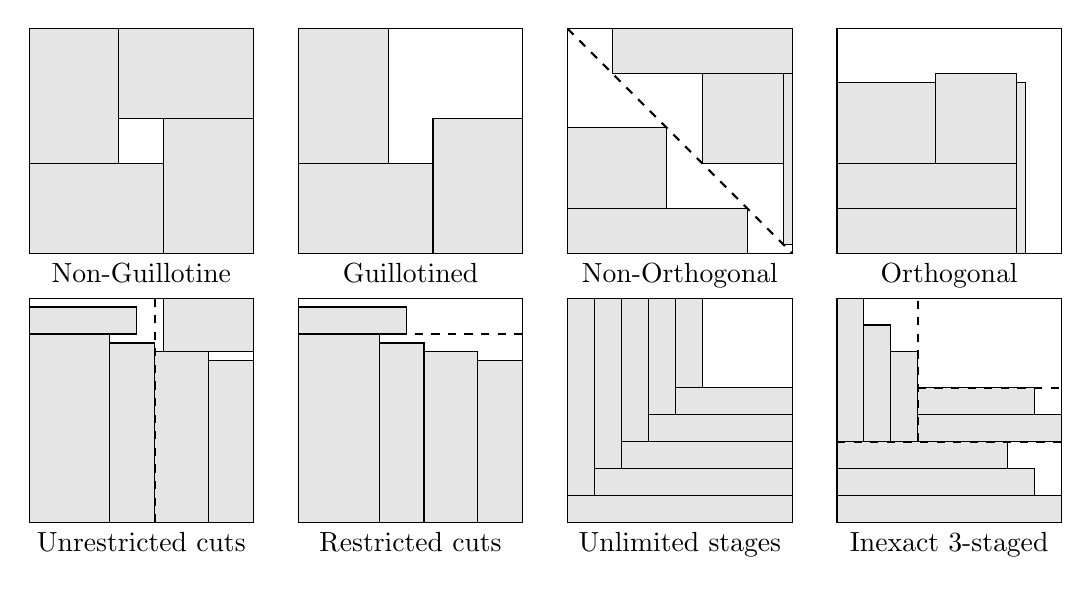
\begin{tikzpicture}[scale=0.114]
\def\piececolor{gray!20}
\def\labelxshift{12.5}
\def\labelyshift{0}
\def\labelfontsize{\normalsize}
\begin{scope}[shift={(0, 0)}] % FIRST ROW
\begin{scope}[shift={(0, 0)}] % FIRST IMAGE
\draw (0,0) rectangle +(25, 25);
\draw[fill=\piececolor] (0, 0) rectangle +(15, 10);
\draw[fill=\piececolor] (15, 0) rectangle +(10, 15);
\draw[fill=\piececolor] (0, 10) rectangle +(10, 15);
\draw[fill=\piececolor] (10, 15) rectangle +(15, 10);

\node [below] at (\labelxshift, \labelyshift) {\labelfontsize Non-Guillotine};
\end{scope}

\begin{scope}[shift={(30, 0)}] % SECOND IMAGE
\draw (0,0) rectangle +(25, 25);
\draw[fill=\piececolor] (0, 0) rectangle +(15, 10);
\draw[fill=\piececolor] (15, 0) rectangle +(10, 15);
\draw[fill=\piececolor] (0, 10) rectangle +(10, 15);
%\draw[fill=\piececolor] (10, 10) rectangle +(15, 10);

\node [below] at (\labelxshift, \labelyshift) {\labelfontsize Guillotined};
\end{scope}

\begin{scope}[shift={(60, 0)}] % THIRD IMAGE
\draw (0,0) rectangle +(25, 25);
\draw[fill=\piececolor] (0,0) rectangle +(20, 5);
\draw[fill=\piececolor] (0,5) rectangle +(11, 9);
\draw[fill=\piececolor] (5, 20) rectangle +(20, 5);
\draw[fill=\piececolor] (15, 10) rectangle +(9, 10);
\draw[fill=\piececolor] (24, 1) rectangle +(1, 19);

\draw[dashed, thick, black] (0, 25) -- (25, 0);

\node [below] at (\labelxshift, \labelyshift) {\labelfontsize Non-Orthogonal};
\end{scope}

\begin{scope}[shift={(90, 0)}] % FOURTH IMAGE
\draw (0,0) rectangle +(25, 25);
\draw[fill=\piececolor] (0,0) rectangle +(20, 5);
\draw[fill=\piececolor] (0, 10) rectangle +(11, 9);
\draw[fill=\piececolor] (0, 5) rectangle +(20, 5);
\draw[fill=\piececolor] (11, 10) rectangle +(9, 10);
\draw[fill=\piececolor] (20, 0) rectangle +(1, 19);

\node [below] at (\labelxshift, \labelyshift) {\labelfontsize Orthogonal};
\end{scope}
\end{scope}

\begin{scope}[shift={(0, -30)}] % SECOND2 ROW
\begin{scope}[shift={(0, 0)}] % FIRST IMAGE
\draw (0,0) rectangle +(25, 25);

%\draw[fill=\piececolor] (0,0) rectangle +(6, 19);
%\draw[fill=\piececolor] (6,0) rectangle +(5, 18);
\draw[fill=\piececolor] (14,0) rectangle +(6, 19);
\draw[fill=\piececolor] (20,0) rectangle +(5, 18);
\draw[fill=\piececolor] (0,0) rectangle +(9, 21);
\draw[fill=\piececolor] (9,0) rectangle +(5, 20);
%\draw[fill=\piececolor] (0,19) rectangle +(10, 6);
\draw[fill=\piececolor] (15,19) rectangle +(10, 6);
\draw[fill=\piececolor] (0,21) rectangle +(12, 3);

\draw[dashed, thick, black] (14, 0) -- (14, 25);

\node [below] at (\labelxshift, \labelyshift) {\labelfontsize Unrestricted cuts};
\end{scope}

\begin{scope}[shift={(30, 0)}] % SECOND IMAGE
\draw (0,0) rectangle +(25, 25);

%\draw[fill=\piececolor] (0,0) rectangle +(6, 19);
%\draw[fill=\piececolor] (6,0) rectangle +(5, 18);
\draw[fill=\piececolor] (14,0) rectangle +(6, 19);
\draw[fill=\piececolor] (20,0) rectangle +(5, 18);
\draw[fill=\piececolor] (0,0) rectangle +(9, 21);
\draw[fill=\piececolor] (9,0) rectangle +(5, 20);
%\draw[fill=\piececolor] (0,19) rectangle +(10, 6);
%\draw[fill=\piececolor] (15,19) rectangle +(10, 6);
\draw[fill=\piececolor] (0,21) rectangle +(12, 3);

\draw[dashed, thick, black] (0, 21) -- (25, 21);

\node [below] at (\labelxshift, \labelyshift) {\labelfontsize Restricted cuts};
\end{scope}

\begin{scope}[shift={(60, 0)}] % THIRD IMAGE
\draw (0,0) rectangle +(25, 25);

\draw[fill=\piececolor] (0,0) rectangle +(25, 3);
\draw[fill=\piececolor] (0,3) rectangle +(3, 22);
\draw[fill=\piececolor] (3,3) rectangle +(22, 3);
\draw[fill=\piececolor] (3,6) rectangle +(3, 19);
\draw[fill=\piececolor] (6,6) rectangle +(19, 3);
\draw[fill=\piececolor] (6,9) rectangle +(3, 16);
\draw[fill=\piececolor] (9,9) rectangle +(16, 3);
\draw[fill=\piececolor] (9,12) rectangle +(3, 13);
\draw[fill=\piececolor] (12,12) rectangle +(13, 3);
\draw[fill=\piececolor] (12,15) rectangle +(3, 10);

\node [below] at (\labelxshift, \labelyshift) {\labelfontsize Unlimited stages};
\end{scope}

\begin{scope}[shift={(90, 0)}] % FOURTH IMAGE
\draw (0,0) rectangle +(25, 25);
\draw[fill=\piececolor] (0,0) rectangle +(25, 3);
%\draw[fill=\piececolor] (0,3) rectangle +(3, 22);
\draw[fill=\piececolor] (0,3) rectangle +(22, 3);
%\draw[fill=\piececolor] (3,6) rectangle +(3, 19);
\draw[fill=\piececolor] (0,6) rectangle +(19, 3);

\draw[fill=\piececolor] (0,9) rectangle +(3, 16);
\draw[fill=\piececolor] (9,9) rectangle +(16, 3);
\draw[fill=\piececolor] (3,9) rectangle +(3, 13);
\draw[fill=\piececolor] (9,12) rectangle +(13, 3);
\draw[fill=\piececolor] (6,9) rectangle +(3, 10);

\draw[dashed, thick, black] (0, 9) -- (25, 9);
\draw[dashed, thick, black] (9, 9) -- (9, 25);
\draw[dashed, thick, black] (9, 15) -- (25, 15);

\node [below] at (\labelxshift, \labelyshift) {\labelfontsize Inexact 3-staged};
\end{scope}
\end{scope}
\end{tikzpicture}

